\documentclass{beamer}
 
\usepackage[utf8]{inputenc}
\usepackage{graphicx}
\usepackage{textcomp}
\newcommand{\textapprox}{\raisebox{0.5ex}{\texttildelow}}

\setbeamertemplate{navigation symbols}{}
\usetheme{Luebeck}

\newcommand\pro{\item[$+$]}
\newcommand\con{\item[$-$]}
%-------------------------------------------------------
%	TITLE PAGE
%-------------------------------------------------------
\title[GEANT4-GPU (McMaster University)]{Running GEANT4 Functions on a GPU}
\subtitle{Discussion of Results}
\institute{McMaster University}
\author[S. Douglas, R. Gorrie, M .Pagnan, V. Reginato]{
Stuart Douglas -- dougls2
\\Rob Gorrie -- gorrierw
\\Matthew Pagnan -- pagnanmm
\\Victor Reginato -- reginavp
}
 
\begin{document}

\frame{\titlepage}
\begin{frame}
\frametitle{Overview}
\tableofcontents
\end{frame}

% =================== Section =================== 
\section{Introduction} 

\subsection{Brief Project Overview}
\begin{frame}
\frametitle{Brief Project Overview}
Take an existing particle simulation toolkit - GEANT4 - and have some functions run on a GPU device to improve performance.
\begin{block}{Definition: GEANT4}
GEANT4 is 
\end{block}
\end{frame}

\subsection{Explanation of Terms}
%Victor
\begin{frame}
\frametitle{What is GEANT4}
\begin{itemize}
\item Geant4 is a toolkit that is meant to simulate the passage of particles through matter. 
\item It has been developed over the years through collaborative effort of many different institutions and individuals. 
\item Geant4 has many different applications, including applications in high energy physics, space and radiation, medical. 
\end{itemize}
\end{frame}

\begin{frame}
\begin{itemize}
\frametitle{What is GP-GPU}
\item General purpose graphic processing unit computing is a re-purposing of graphics hardware
\item Allows GPUs  to perform computations that would typically be computed on the CPU
\item If problems are suitable to mass parallelization 
\end{itemize}
\end{frame}

\subsection{Scope}
\begin{frame}
\frametitle{Scope}
\end{frame}

\subsection{Purpose}
\begin{frame}
\frametitle{Purpose}
\end{frame}


% =================== Section =================== 
\section{Features}
\subsection{GPU acceleration done behind the scenes}
\begin{frame}
\frametitle{GPU acceleration done behind the scenes}
\begin{itemize}
\item Old projects can be run using GPU acceleration with out having to change anything 
\item No new functions to learn
\end{itemize}
\end{frame}

\subsection{Able to build GEANT4 with GPU on or off}
\begin{frame}
\frametitle{Able to build  GEANT4 with GPU on or off}
\end{frame}

\section{Particle Simulations on GPU}
\begin{frame}
\frametitle{Why G4ParticleHPVector}
\end{frame}

\begin{frame}
\frametitle{Two Implementations}
\begin{itemize}
\item Run everything on the GPU
\item Only select functions run on GPU
\end{itemize}
\end{frame}

\subsection{Entire G4ParticleHPVector Object on GPU}
\begin{frame}
\frametitle{Completely on GPU}
\begin{itemize}
\item The vector is stored exclusively on the GPU
\pro Do not have to maintain a copy of the vector on the CPU
\pro Do not have to maintain the hashed vector
\pro Reduces how much is being copied to the GPU
\con All functions are run on the GPU
\end{itemize}
\end{frame}

\subsubsection{Intensive Functions on GPU}
\begin{frame}
\frametitle{Intensive Functions on GPU}
\end{frame}

\subsubsection{Performance}
\begin{frame}
\frametitle{Performance Results}
\end{frame}

\begin{frame}
\frametitle{Performance Discussion}
\end{frame}

\subsubsection{Accuracy}
\begin{frame}
\frametitle{Accuracy}
\end{frame}

\subsubsection{Testing}
\begin{frame}
\frametitle{Testing}
\end{frame}

\subsection{Implementation 2}
\begin{frame}
\frametitle{Implementation 2}
\begin{itemize}
\pro Only functions that run faster on the GPU are implemented
\pro Not forced to run functions that run slowly on GPU
\con Will have to maintain two copies of the vector
\con More copying the vector to and from the GPU
\end{itemize}
\end{frame}

\subsubsection{Performance}
\begin{frame}
\frametitle{Performance Summary}
\begin{itemize}
\item Most functions slower on GPU until \textapprox 10,000 entries 
\item Most \emph{commonly-used} functions significantly slower on GPU
\begin{itemize}
\item Lots of data accesses
\end{itemize}
\item Many problems in vector class not well-suited to parallelism
\end{itemize}
\end{frame}

\begin{frame}
\frametitle{Performance Results - \texttt{Times}}
\begin{itemize}
\item Multiplies each point in vector by factor
\end{itemize}
\begin{figure}
\centering
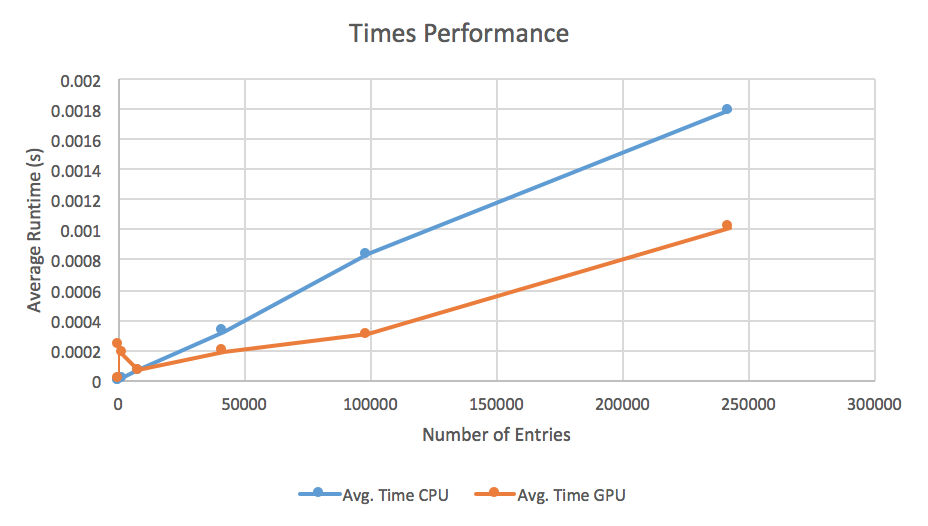
\includegraphics[width=0.9\textwidth]{images/times_line.png}
\caption{Runtime vs. Number of Data Points -- \texttt{Times}}
\end{figure}
\end{frame}

\begin{frame}
\frametitle{Performance Discussion}
\end{frame}

\subsubsection{Accuracy}
\begin{frame}
\frametitle{Accuracy}
\end{frame}

\subsubsection{Testing}
\begin{frame}
\frametitle{Testing}
\end{frame}

\section{Conclusion}
\subsection{Summary of Results}
\begin{frame}
\frametitle{Summary of Results}
\end{frame}

\subsection{Recommendations}
\begin{frame}
\frametitle{Recommendations}
\end{frame}

\end{document}